%File: formatting-instruction.tex
\documentclass[letterpaper]{article}
\usepackage{aaai}
\usepackage{times}
\usepackage{helvet}
\usepackage{courier}
\usepackage{float}
\usepackage{hyperref}
\frenchspacing
\usepackage{graphicx}
\graphicspath{ {./images/} }
\setlength{\pdfpagewidth}{8.5in}
\setlength{\pdfpageheight}{11in}
\pdfinfo{
/Title (Increase Efficiency and Reliability in Hospital Emergency Rooms using Human Robot Interaction - An Application)
/Author (Cecilia Aponte)}
\setcounter{secnumdepth}{0}  
 \begin{document}
% The file aaai.sty is the style file for AAAI Press 
% proceedings, working notes, and technical reports.
%
\title{Increasing the Efficiency and Reliability in Hospital Emergency Rooms using Human Robot Interaction - An Application}
\author{Cecilia Aponte\\
Masters of Science in Engineering in Artificial Intelligence and Robotics\\
Human Robot Interaction (HRI)\\
Sapienza Universita di Roma\\
ID: 1822225\\
}
\maketitle
\begin{abstract}
\begin{quote}
Hospital Emergency Rooms (ER) suffer of many deficiencies that cause issues such as overcrowding, possible malpractice, and even mortality. To reduce and potentially remove these issues, technology such as robots can be implemented at the beginning of the process. The robot in this implementation is capable of interacting with humans using a software that also simplifies the process of adding new patients into the database with information regarding their emergency, it provides an urgency level calculated based on the entered information, and their estimated wait time. Patients can also return to the robot at any time to ask for their remaining wait time and update their information (e.g. symptoms, pain level) in case their emergency worsens and could require a more urgent appointment and a faster evaluation from a doctor. For a new patient or an existing one that has a high level urgency, their appointment is calculated to be shorter in order to avoid the possibility of malpractice or mortality due to extended wait time for potentially dangerous circumstances. On the other hand, patients with lower urgency level are taken in order, but are communicated if their wait time has changed due to other urgent priorities. This increased direct communication with the patients reduces the stress and confusion with both patients and practitioners. Therefore, increasing the efficiency and reliability of the most important step in the ER - prioritization of patients given the severity of their symptoms and pain level and the correct initial calculation of their urgency level.
\end{quote}
\end{abstract}

\section{Introduction}
\noindent 
Technology has helped improve many aspects of our daily life from communication to transportation to health and further. Nowadays, our health has progressed due to advancements in medical procedures, drugs, devices, etc. However, one area that has been left without significant advancement is the upgrade in patient care during the arrival of a new patient to the hospital. Emergency rooms across the world face the same issues regarding lack of: personnel, structure and order, capacity, technology, and other inefficiencies. Many of these issues can be resolved by employing a robot with the capacity of interacting with humans and improve the throughput of the ER patient resolution process.\\

Some of the main complaints given by patients after their experience in an ER are: the amount of time waited to be checked or asked about their symptoms to access the emergency's urgency, total wait time in the ER, lack of information about their estimated wait time, lack of check-ups by any staff, noticing patients that arrived after and/or have a less critical emergency are taken care of faster (potentially due to these patients being the 'loudest' and complaining to staff constantly to be checked, which unfortunately leaves those who are worse and cannot or do not press staff about their condition waiting longer and aggravating their circumstances. All of these issues can be resolved through this robot Intelligent system and HRI:   

\begin{itemize}
\item Patients are entered into the database as soon as they enter the ER. Patients or anyone accompanying them interacts with the robot to add the patient's information and their emergency data.
\item The total wait time in the ER is reduced due to an efficient prioritization of patients given their urgency levels. Higher urgency patients can be taken care of first, which reduces the possibility of further complications due to extended wait time. This in turn shortens their length of stay in the hospital, and therefore decreases overcrowding.
\item Patients have total control to check their remaining wait time at any moment. Improving communication and confidence in the reliability of the hospital and their customer service.
\item Patients can update their record information with any changes in their emergency, therefore granting custom check-ups as deemed by the patients and recalculation of urgency level and wait time if their symptoms worsen. 
\item Emergencies are categorized due to their urgency, so any changes in the order of appointments are solely calculated through the software. 
\end{itemize}

The robot used in this implementation is called MARRtino, a ROS-based low-cost differential drive robot platform created by the Artificial Intelligence and Robotics department in Sapienza University in Rome, Italy. The robot is capable of smart navigation, spoken human-robot interaction, image analysis, among others and is used in a variety of educational activities, ranging from pre-school children to PhD and PostDoc in the field.\\

To execute this HRI system, a multi-modal interaction (structure used to describe high-level interactions) is used for the dialogue mechanism. Spoken dialogue is enabled through speakerphones and microphone (for the possibility of speech recognition from the patient to the robot) and virtual interaction through a tablet for button touch responses. The robot system can be found in \href{https://github.com/ccapontep/HumanRobotInteraction_ER}{GitHub:HRI-ER} for all the resources. \\

\section{HRI System Structure}
The HRI system starts by presenting the patient with two options, either a new or existing patient. The new patient will be introduced to the system and asked to enter the information regarding their emergency. The existing patient can has the option to either check their remaining wait time or to update their record in case new or worsening symptoms. 

\subsection{New Patient}
When the new patient enters the hospital ER, they are given a physical ticket with their number to be entered into the database. This will also help the patient remember their patient record number. As the patient enters the ER room, the robot will welcome them through the tablet and ask for their interaction. A series of questions are prompted to be answered by the patient:

\begin{itemize}
\item Name - enter first and last names
\item Age - enter current age
\item Medical History - usual patient's past history such as diabetes, high-cholesterol, or recurring symptoms
\item Emergency Symptoms - includes the most severe symotoms that could risk the patient's life such as 'bleeding that does not stop', sudden severe pain', 'deep or large wound', 'feeling of committing suicide or murder'
\item General Symptoms - includes symptoms such as fever, pain, inflammation
\item Location of Pain(s) - includes each general part of the body 
\item Level of Consciousness - from fully awake to unconscious
\item Pain Level - from some to excruciating
\item Time and Date Admitted - automatically added after finalizing the questionnaire
\end{itemize}

\begin{figure}
  \centering
  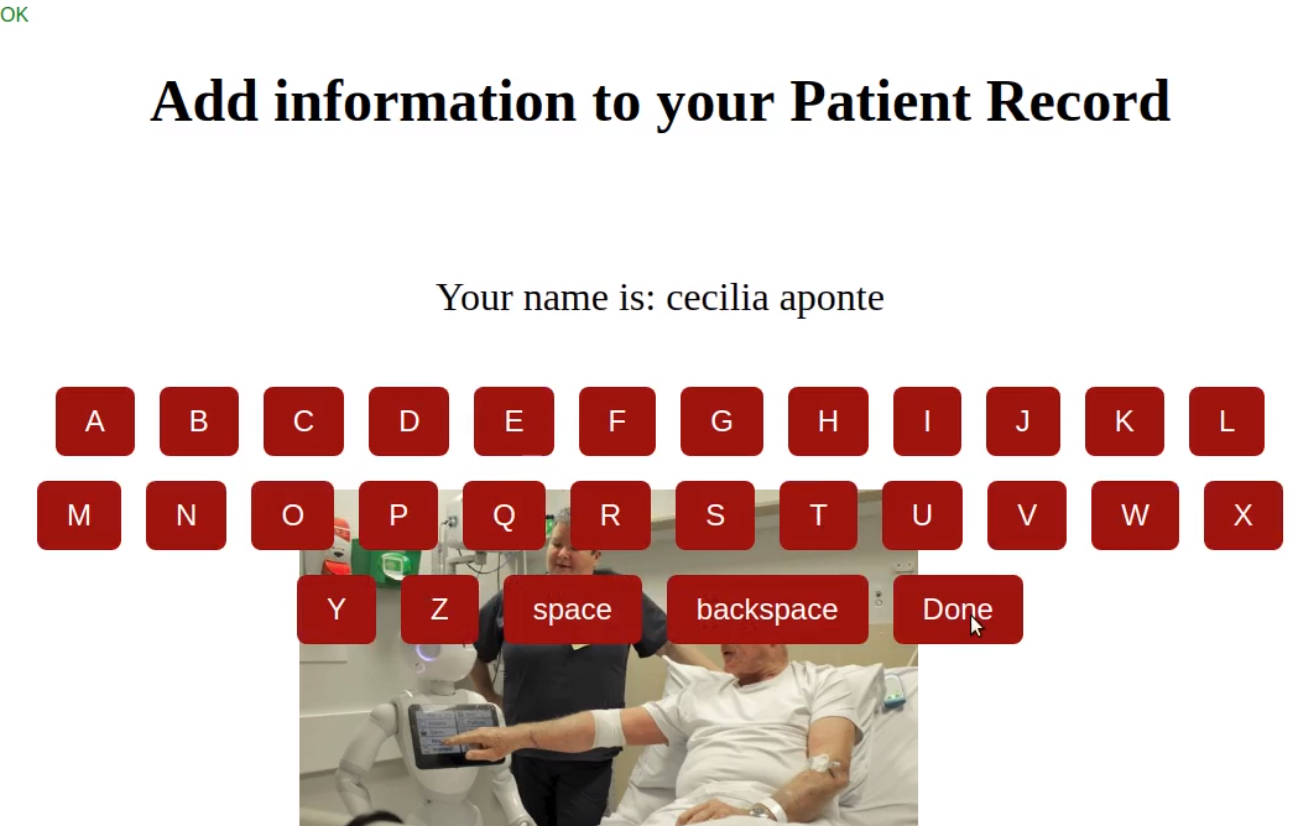
\includegraphics[width=.45\textwidth]{RecordAddName.png}\hfill
  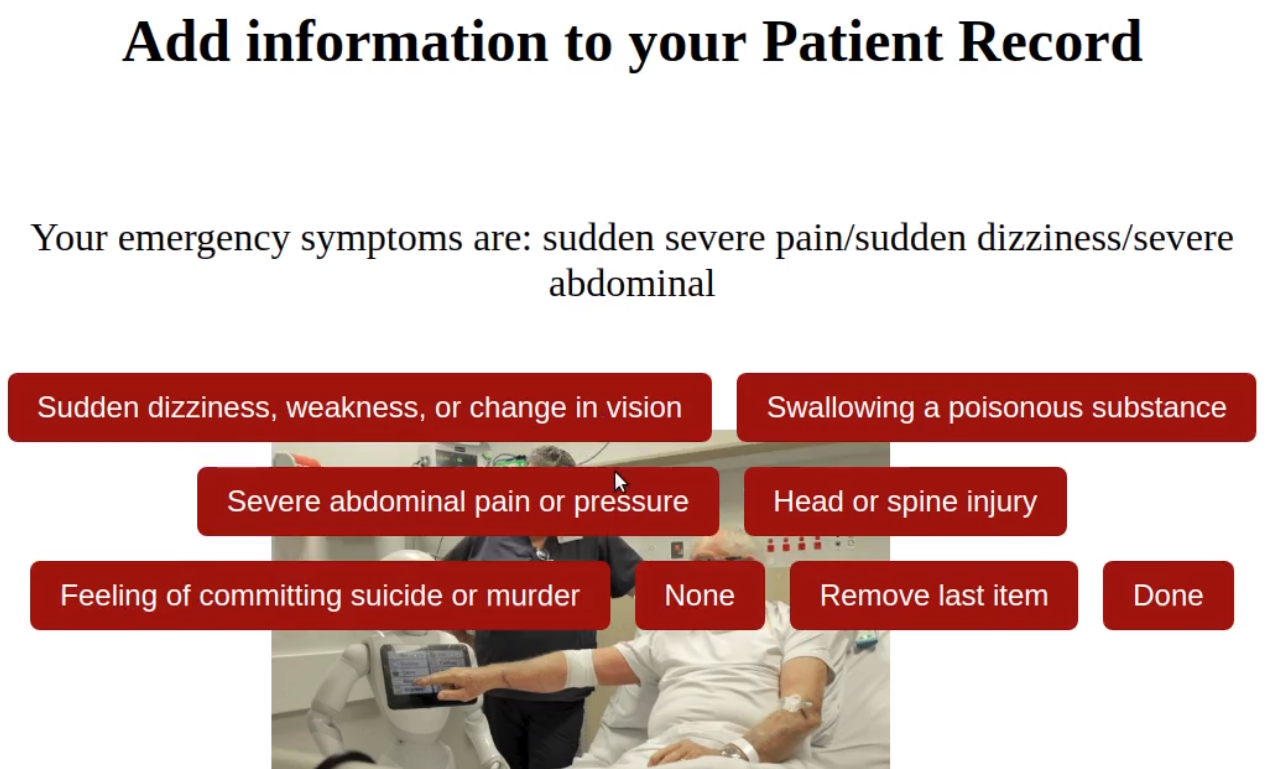
\includegraphics[width=.45\textwidth]{RecordAddEmergencyMain.png}\hfill
  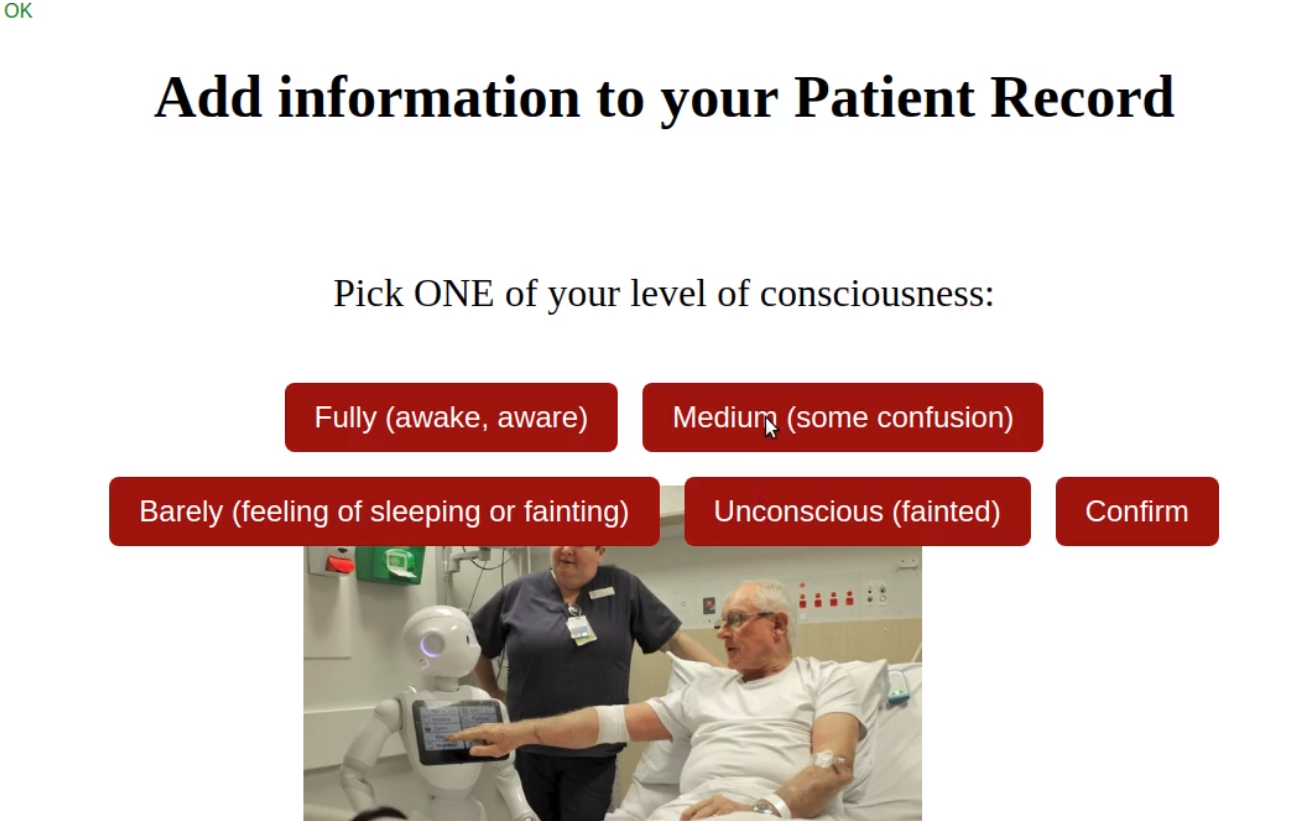
\includegraphics[width=.45\textwidth]{RecordAddConsciousness.png}\hfill
  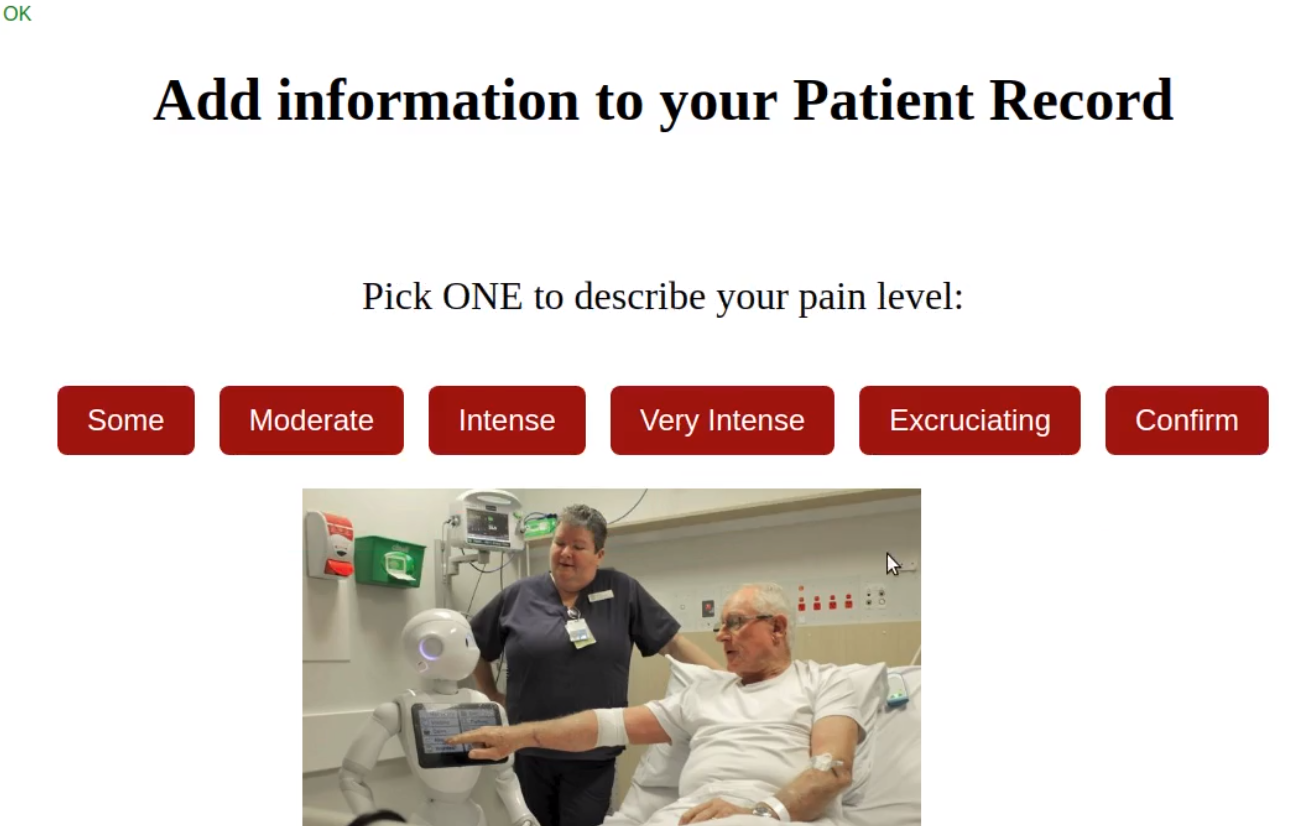
\includegraphics[width=.45\textwidth]{RecordAddPainLevel.png} \bigskip 
   \caption{Interaction through the tablet asking the user to add (from top to bottom): name, emergency symptoms, consciousness, and pain level.} 
\end{figure}


\subsection{Urgency Level}

The robot system contains a method to calculate the urgency level of the patients given the information entered in the database. The general point system is given by the following:

\begin{itemize}
\item For the age, patients that are younger than 10 years are given the highest points since they are more fragile than an adult. Patients older than 70 are given the next higher points since at that age any urgency is very delicate to treat.

\item For past medical history, each item picked adds some points. If the user specifically smokes and has any chest pain as a symptom or location. Each of these can also be later expanded to include specific dangerous scenarios with the help of a medical practitioner.

\item Pain level is given points by the severity. From \textit{some} to \textit{intense}, there is one point difference in each. However from \textit{very intense} to \textit{excruciating}, there are two points difference to extenuate their importance.

\item The points for the emergency symptoms are calculated by multiplying each of these symptoms by a point quantity and later also multiplied by the pain level. This way it is defined as a high emergency symptom with the high points and with the severity of the pain level.

\item The general symptoms are calculated using the same method than the emergency symptoms, however the point quantity that it is multiplied with is much lower.

\item Location of the pain given by a normal area is given by a lower point for each location added. On the other hand, the more delicate areas like the \textit{abdomen, chest,} or \textit{head} has a slightly higher point.

\item For the consciousness points, the \textit{medium} has a low point, the \textit{barely} has much higher point, and \textit{unconscious} has the highest points.
\end{itemize}

All these points are added and then are defined as low, medium and high priority depending on their point range category.

\begin{figure}
  \centering
  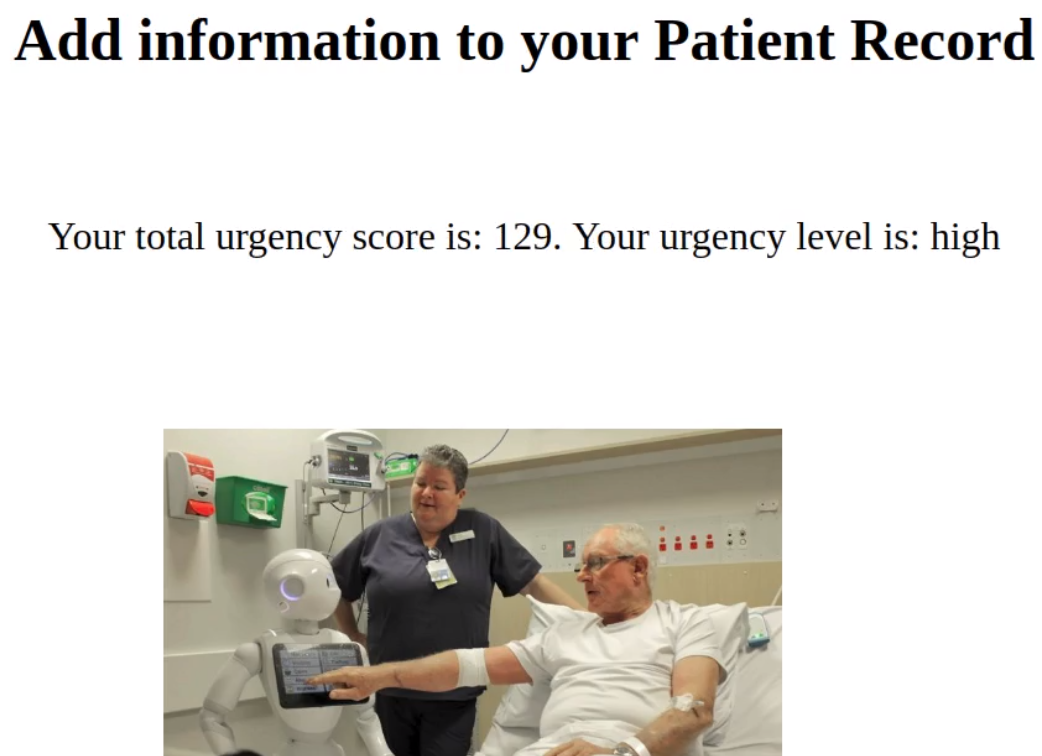
\includegraphics[width=.35\textwidth]{RecordUrgencyScore.png}\hfill
   \caption{Total score given by all the information added by the patient into the system.}
\end{figure}

\subsection{Wait Time}
The wait time for the patient is calculated depending on the other patients already waiting and everyone's urgency level. Each patient is given 15 minute-appointment with the doctor who will examine them and diagnose them. Each new patient that enters the ER can be placed in front of the queue of another person only if their urgency score is at least 10 points higher than that person and has at least a higher-medium score. Meaning that the incoming patient has to have a high urgency level, otherwise it has to remain behind the queue.\\

Once the new wait time for the patient is calculated, its order on the new queue is evaluated. Likewise, the wait time and order of the rest of the patients waiting are calculated and saved in their records as seen in Figure 4. Each patient that has been affected with a patient being moved in front of them in the queue is communicated so when they query their record (see next section).

\begin{figure}
  \centering
  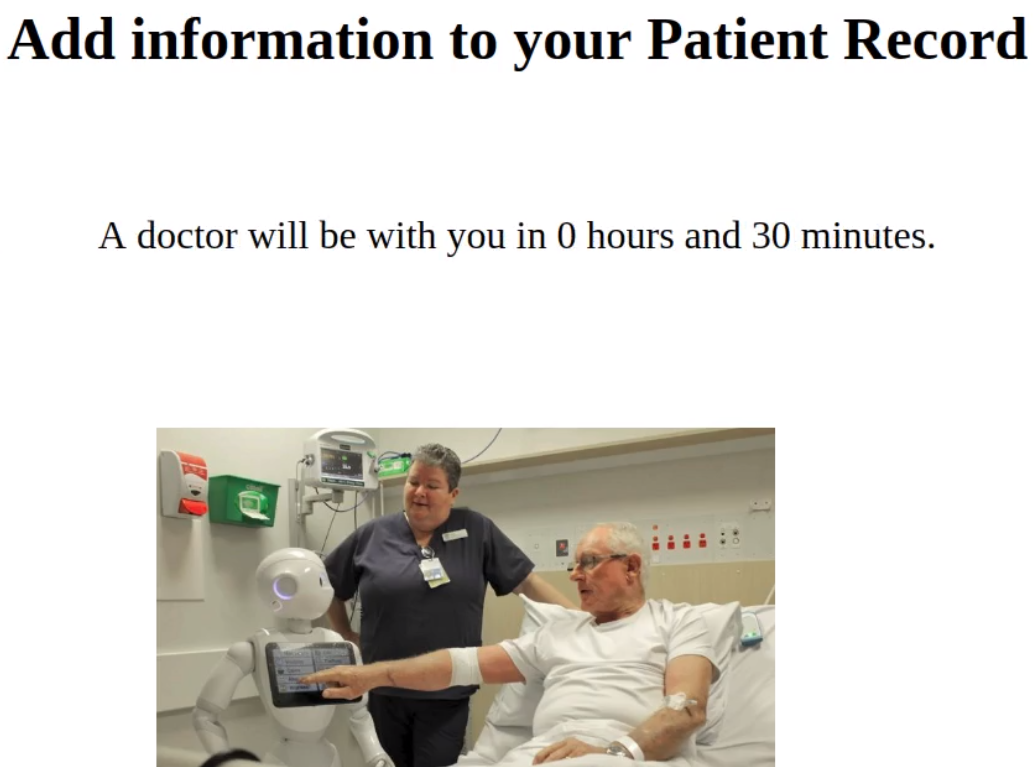
\includegraphics[width=.35\textwidth]{RecordWaitTime.png}\hfill
   \caption{Shows the wait time calculated for the new patient.}
\end{figure}

\begin{figure}
  \centering
  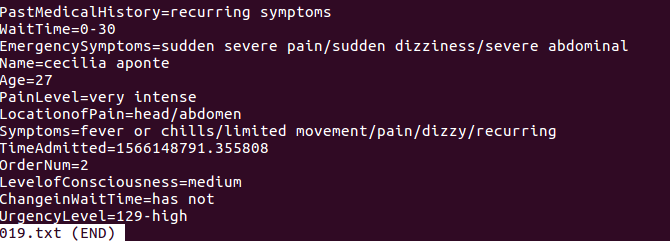
\includegraphics[width=.35\textwidth]{RecordNew019-Aponte.png}\hfill
   \caption{Record saved in the databases of the new patient.}
\end{figure}

\subsection{Returning Patient}
The patient that has been already added to the database can also interact with the robot system. They have two options, get their remaining wait time to be checked by a doctor and/or update their symptoms in case they have changed in form or severity. The user can check as many times as needed.\\

\begin{figure}[H]
  \centering
  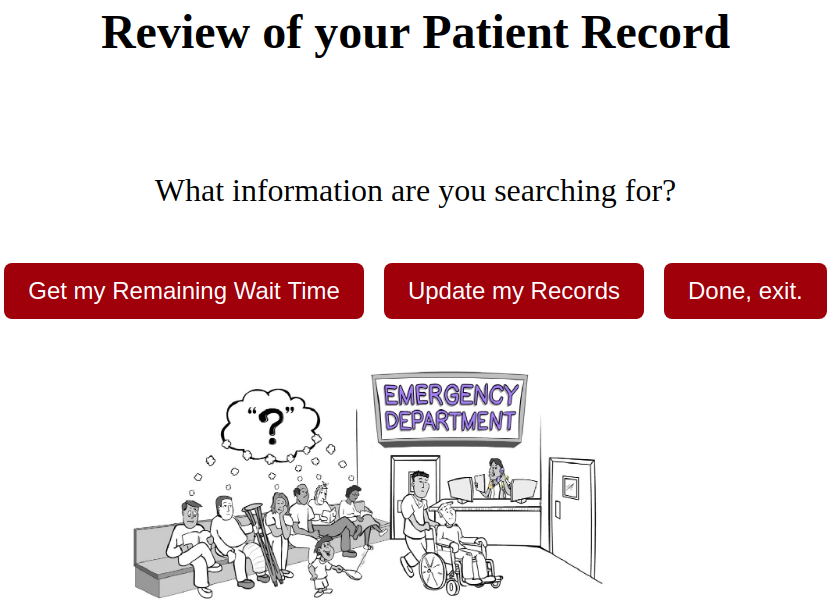
\includegraphics[width=.35\textwidth]{ReviewRecordChoose.png}\hfill
   \caption{Shows the options the returning patient can choose from.}
\end{figure}

\begin{itemize}
\item Remaining wait time: is calculated by the difference at the moment the user makes the query and the record that contains the date admitted.


\begin{figure}[H]
  \centering
  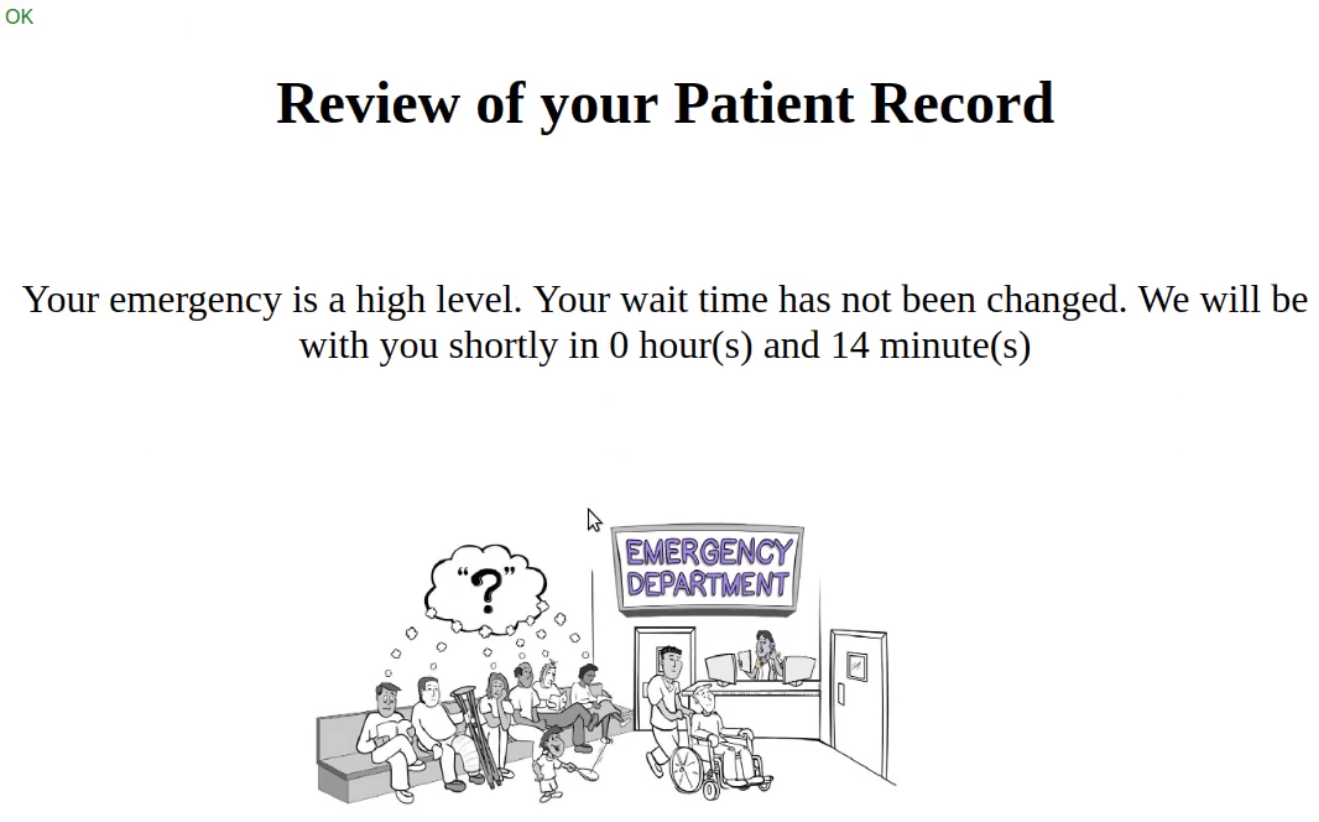
\includegraphics[width=.35\textwidth]{RemainWaitTime.png}\hfill
   \caption{Reply from the robot system about the time remaining to be seen by the medical practitioner.}
\end{figure}

\item Update symptoms: the patient can change the following sections in their record to update any changes in their emergency: \textit{emergency symptoms, symptoms, location of pain, level of consciousness, and pain level.} After all changes are done and the patient exits the system, their urgency score is recalculated. If their score has increased by at least 10 points and has a high urgency level, their order in the queue and wait time are recalculated. This recalculation is done with the same requirements as described in the section Wait Time above.

\end{itemize}


\begin{figure}[H]
  \centering
  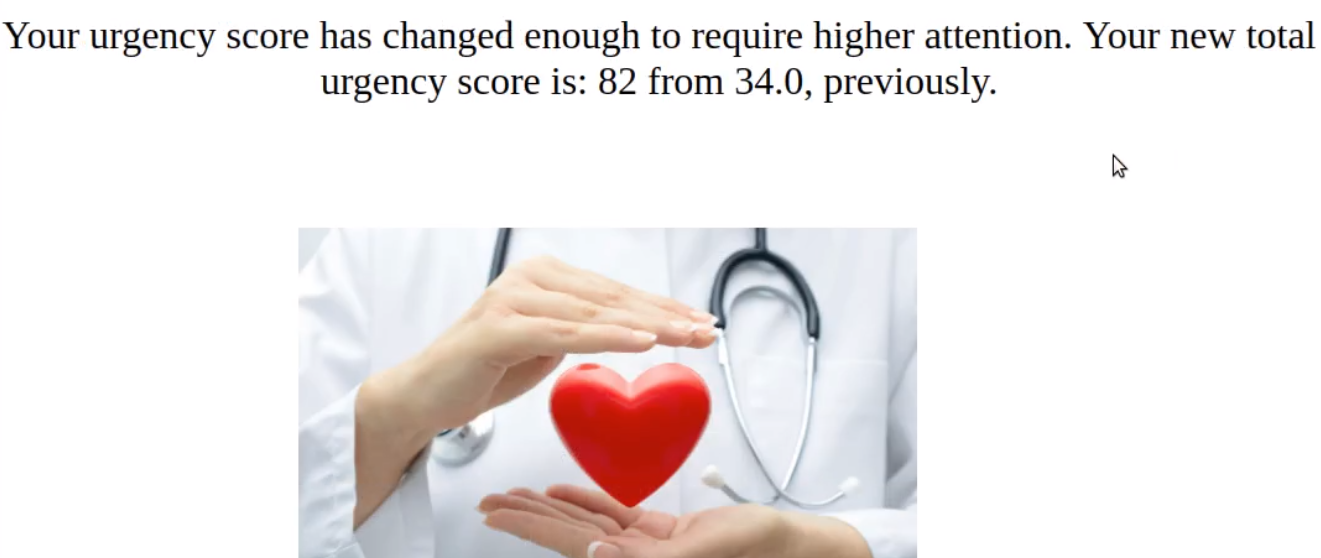
\includegraphics[width=.35\textwidth]{ChangeUrgencyScore-012.png}\hfill
  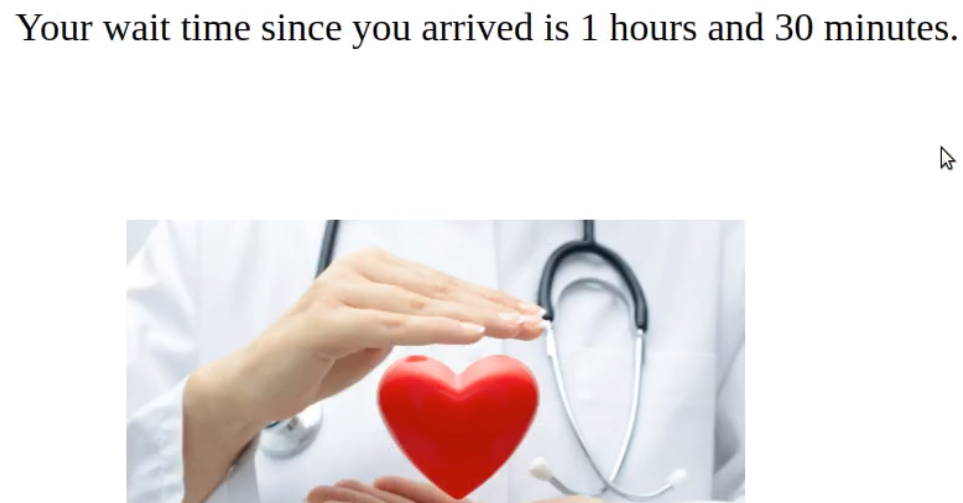
\includegraphics[width=.35\textwidth]{ChangeWaitTime-012.png}\hfill 
   \caption{The patient gets information about their new score and new wait time, if their score has surpassed the described criteria.}
\end{figure}

\begin{figure}[H]
  \centering
  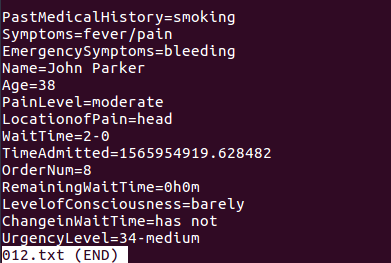
\includegraphics[width=.25\textwidth]{RecordChange012-before.png}\hfill
  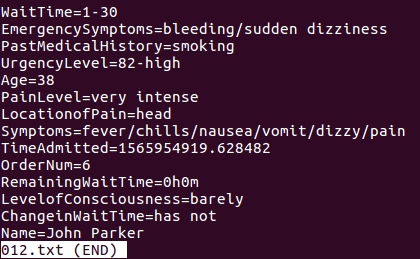
\includegraphics[width=.25\textwidth]{RecordChange012-after.png}\hfill \caption{The patient's record also shows the updates of the picked items and also the new urgency score and level, wait time, and order in the queue.}
\end{figure}

\subsection{Results}
When testing with real scenarios, the robot system performs as needed. Two scenarios are described below to test the accuracy, reliability, and interaction of the system with possible patients. 

\subsubsection{Scenario 1: Patient with Appendicitis}
A subject that has previously experienced appendicitis and enters the ER showing the usual symptoms and pain levels is given a high urgency score. This is the correct action, since if an appendicitis is not treated promptly it can result in death. Therefore, the quick first guess about the severity given the robot system helps the ER personnel give attention to these type of patients, as well as any other high-risk individuals. 

As the same patient finds themselves having symptoms that worsen, they input their new emergency information to the system. The robot system then correctly reevaluates the change and returns a higher urgency score and their new order in the queue. In a real ER, this individual would probably be left with worsening symptoms and an increasing risk of peritonitis (bursting of the appendix) and potential death without any medical practitioner knowing or acknowledging. With this system, the ER staff does not have to worry about being saturated with patients always complaining but unable to know the order of each patient and if one requires more attention. The main way this happen usually is if the patient or their family/friends are bringing more attention to that patient. Therefore \textit{'the loudest are taken care of first'} is removed and replaced by a more precise and reliable system that depends more on the facts and communication with the patients.

\begin{figure}[H]
  \centering
  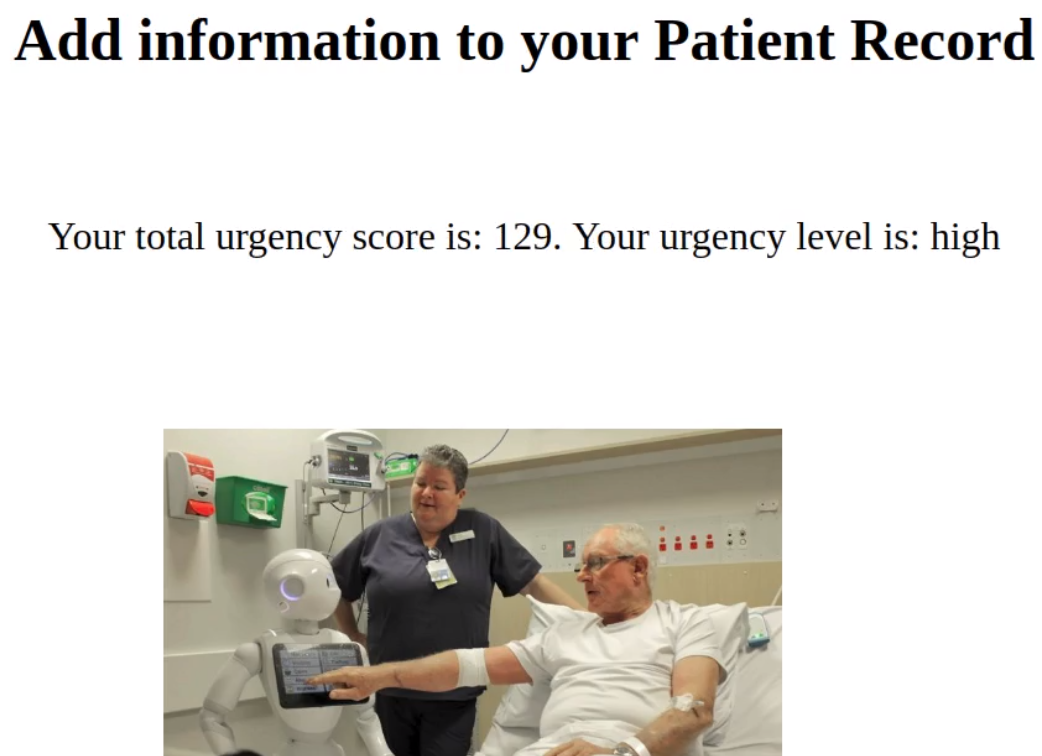
\includegraphics[width=.25\textwidth]{RecordUrgencyScore.png}\hfill
  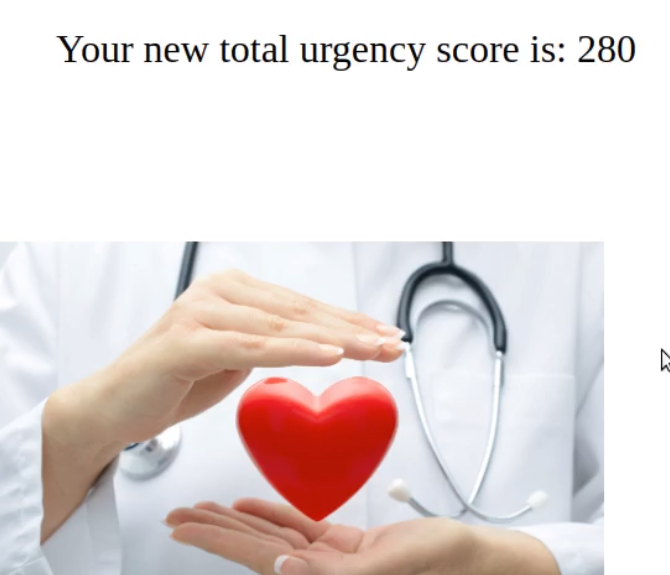
\includegraphics[width=.2\textwidth]{NewUrgencyScore.png}\hfill 
   \caption{The patient experiencing appendicitis is given correctly a high urgency score and level. When they then experience worse symptoms, the system recalculates their new urgency score and level, wait time, and order in the queue.}
\end{figure}

\subsubsection{Scenario 2: Direct experience with the robot system}
Two users tested the interaction with the robot using a real scenario they experienced in their past that took them to the ER. Each user was only given general information about the goal of the robot. Their interaction was recorded fully without providing any guidance. This was done to see the raw experience of the user like a new patient would when entering the ER. A video was created with the collection of these results for the application of the HRI system. \\

One issue was seen with the system clearly at the beginning, as was expected. Since the robot is smaller than a regular-sized adult, the users had to either squat or bend over to reach the tablet buttons. This also complicated the angle with which the user could touch the buttons properly. This was expected previous to testing, as in general it is common to find robots smaller in size than humans. To aid this issue, the system can include spoken language detection so the user can just speak the responses. The MARRtino robot does have Automatic Speech Recognition (ASR) capabilities. \\

The remaining of the interactions with the users were satisfactory. The system led the user from the beginning to the end entering the information properly and providing the information that any patient would have in the ER. In addition to check-ups that are necessary for patients such as remaining wait time and changes in the type and/or severity of their symptoms. \\

Both users had positive feedback after concluding the interaction. They affirmed the robust simplification of a complex, delicate situation as is the health of a patient entering an ER. The system surpassed their expectations and found the use very important and necessary in all hospitals. 


\section{Future Work}
Several improvements can be added to the system to improve its design and results, so that it could progress in its robustness. 

\begin{itemize}
\item Language: one very useful detail that can be expanded to the robot is the possibility of functioning with different main languages such as Spanish. In main cities such as Rome, Italy there are a high quantity of immigrants and tourists. Their lack of knowledge of the native language can make it almost impossible to communicate with the hospital staff. Adding this flexibility would aid many people in hospitals in this globalized world.

\item Check-ups: robots can physically check-up on the patients every so often (e.g. 30 minutes) to query any patient that might need help with anything. The MARRtino robot does have this capability, as do many robots.

\item Doctor placements: the robot can coordinate also the information about which doctor each patient will be seeing when they signify they are free. Different doctors can get specific level of urgency, depending on their experience level or just as a rotation. This way, low and medium-urgent patients are handled faster and known beforehand.

\item Robots: 
    \begin{itemize}
    \item The simplest implementation would be to remove the need of a robot. Of course having a robot improves the interaction with a user, since a robot provides a resemblance to a human-human interaction compared to working directly with a software. However the exclusion of a robot could potentially enable a higher deployment of the system in any hospital of the world with minimum resources: kiosks at the entrance of hospitals with this system. The user could even connect to the system from home and add their information previous to arriving, or even wait at home until it is almost time for their appointment (reducing congestion in the ER). This simplification could also include more complex robots doing other tasks, in order to allocate the robots where they will be needed.
    
    \item More human-like robots, like SoftBank's Pepper, can be used at the entrance, so that patients can feel more at ease as they will feel more approachable and technological.
    
    \item Simpler robots, like the MARRtino robot, can be used for check-ups since their aim is to provide a tool for changes and simple communication.
    
    \item Cameras in the waiting area or on the same robots with vision and perception capabilities can be used to determine any sudden change in patients such as fainting, deep bleeding, etc. Also to be able to scan patient's ticket without having to type or speak the ticket numbers.
    
    \item Specialized robots such as Samsung Bot Care Bixby can be implemented to read patient's blood pressure and heart rate.
    
    \item Multi-robot architecture where all these robots are connected to the system database and coordinate changes.
    \end{itemize}
    
\item Robustness: medical questions, diagnosis, and scoring can be setup into the system by acquiring help from experienced medical practitioners. For example, the Emergency Severity Index (ESI) can be implemented. 

\item Diagnosis: using a diagnositc tool in the robot system that can provide a possible diagnosis of the patient's emergency as a method to provide a more accurate scoring. Certainly, the final diagnosis is done by the doctor.

\end{itemize}

\section{Conclusion}
This ER Robot system has been found to have a real, important application to one of the most pressing issues of today. In order to provide an effective and efficient health system, mechanisms such as this are needed. This application is the start of the possibility of necessary and robust changes to take place in hospitals. The system as is can start being used to assess further changes, performance, and reactions with users. As these become more certain and technology keeps improving, further expansion of the quantity of robots used and deployment to different hospital areas such as patient check-ups after their intervention can be handled.

\section{Resources}
The implementation code can be found in the following github: \\ \url{https://github.com/ccapontep/HumanRobotInteraction_ER} \bigskip

\noindent
The video showing the user results can be found at the youtube channel: \href{https://www.youtube.com/channel/UCgLahJX6Fz3qhQzgIl7dD8w?disable_polymer=true}{Create. Robotics.AI.} \bigskip

\noindent
To see the video to the direct link here: \href{https://www.youtube.com/watch?v=B4sg4iSE8-Q}{User Results}

\section{References} 

Di Somma, S., Paladino, L., Vaughan, L. et al. Overcrowding in emergency department: an international issue. Intern Emerg Med (2015) 10: 171.
\\

\noindent Olaronke, Iroju & Ojerinde, Oluwaseun & Ikono, Rhoda. (2017). State Of The Art: A Study of Human-Robot Interaction in Healthcare. International Journal of Information Engineering and Electronic Business. 3. 43-55. 10.5815/ijieeb.2017.03.06. 
\\

\noindent Wilkes, D.M.; Franklin, Stan; Erdemir, Erdem; Gordon, Stephen; Strain, Steve; Miller, Karen; and Kawamura, Kazuhiko. 2010. Heterogeneous Artificial Agents for Triage Nurse Assistance. In \textit{Proceedings of the IEEE-RAS International Conference on Humanoid Robots} Nashville, TN, USA: IEEE Press.


\end{document}